\documentclass[10pt, a4paper]{article} 

\usepackage[T1]{fontenc}
\usepackage[utf8]{inputenc}
\usepackage[british]{babel}  
\usepackage[left = 0mm, right = 0mm, top = 0mm, bottom = 0mm]{geometry}
\usepackage[stretch = 25, shrink = 25, tracking=true, letterspace=30]{microtype}  
\usepackage{graphicx}
\usepackage{xcolor}
\usepackage{fontawesome5}

\usepackage{enumitem}
\setlist{parsep = 0pt, topsep = 0pt, partopsep = 1pt, itemsep = 1pt, leftmargin = 6mm}

\usepackage{FiraSans}
\renewcommand{\familydefault}{\sfdefault}

\definecolor{accent}{HTML}{582900}

%%%%%%% USER COMMAND DEFINITIONS %%%%%%%%%%%%%%%%%%%%%%%%%%%
\newcommand{\dates}[1]{\hfill\mbox{\textbf{#1}}}
\newcommand{\is}{\par\vskip.5ex plus .4ex}
\newcommand{\headleft}[1]{\vspace*{3ex}\textsc{\textbf{#1}}\par%
    \vspace*{-1.5ex}\hrulefill\par\vspace*{0.7ex}}
\newcommand{\headright}[1]{\vspace*{2.5ex}\textsc{\Large\color{accent}#1}\par%
     \vspace*{-2ex}{\color{accent}\hrulefill}\par}
%%%%%%%%%%%%%%%%%%%%%%%%%%%%%%%%%%%%%%%%%%%%%%%%%%%%%%%%%%%%

\usepackage[colorlinks = true, urlcolor = white, linkcolor = white]{hyperref}

\begin{document}

% Style definitions -- killing the unnecessary space and adding the skips explicitly
\setlength{\topskip}{0pt}
\setlength{\parindent}{0pt}
\setlength{\parskip}{0pt}
\setlength{\fboxsep}{0pt}
\pagestyle{empty}
\raggedbottom

\begin{minipage}[t]{0.33\textwidth} %% Left column -- outer definition
%  Left column -- top dark rectangle
%% \colorbox{accent}{\begin{minipage}[t][5mm][t]{\textwidth}\null\hfill\null\end{minipage}}

\vspace{-.2ex} % Eliminates the small gap
\colorbox{accent!90}{\color{white}  %% LEFT BOX
\kern0.09\textwidth\relax% Left margin provided explicitly
\begin{minipage}[t][298mm][t]{0.88\textwidth}
\raggedright
\vspace*{2.5ex}

\Large Évrard \textbf{\textsc{Van Espen}} \normalsize 

% Centering without extra vertical spacing
\null\hfill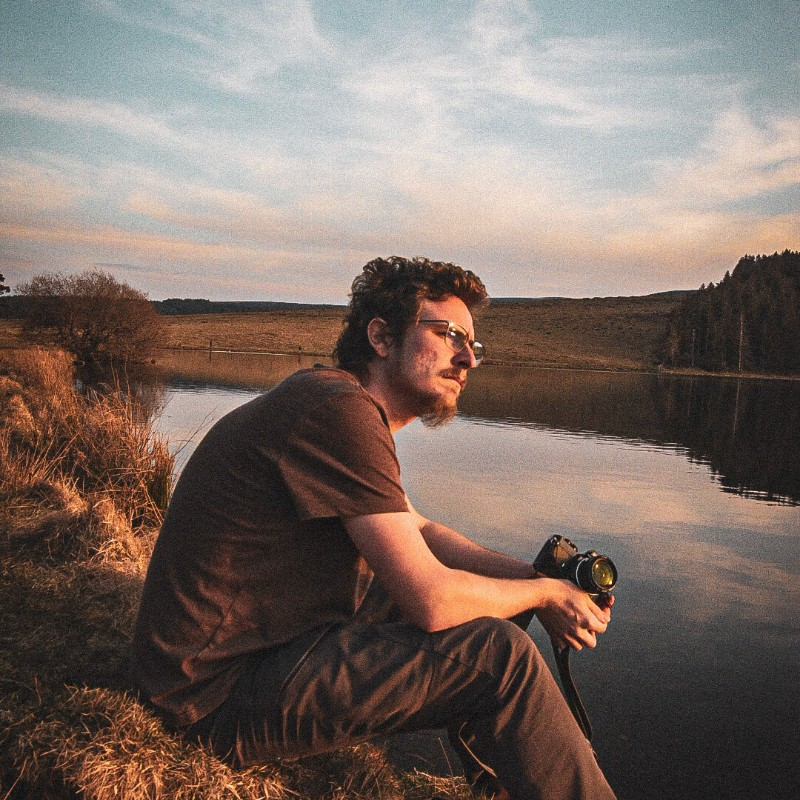
\includegraphics[width=0.65\textwidth]{me.jpeg}\hfill\null

{\small\headleft{Profil}}
{\small
Développeur \textit{full stack} et \textit{devops} expérimenté fort de plusieurs années de travail en \textit{startup}. Mes compétences vont de la réalisation de maquettes et de la conception de l'architecture au développement complet ainsi qu'à la production en conditions opérationnelles en passant par la conduite de réunions et la réalisation de documentations aussi bien techniques qu'à destination des utilisateurs. Compétent en développement \textit{front-end} aussi bien qu'en développement \textit{back-end} et en administration de systèmes \textit{Linux}, de quelques machines à plusieurs dizaines.
}

{\small\headleft{Contact}}
\small
\faAt\ {\small \href{mailto:evrard@vanespen.dev}{evrard@vanespen.dev}} \\
\faPhone \ +33\,7\,81\,29\,99\,59 \\
\faGithub \ \href{https://github.com/evanespen}{evanespen} \\
\faLinkedin \ \small \href{https://www.linkedin.com/in/evrard-van-espen-28a003202}{linkedin.com/in/evrard-van-espen-28a003202}
\normalsize

{\small\headleft{Informations personnelles}}
{\small
Nationalité: \textbf{Française} \\
Localisation: \textbf{Clermont-Ferrand} (remote ou hybride) \\
Langues: \textbf{Français} (natal), \textbf{Anglais} (courant)
}

{\small\headleft{Compétences}}
{\small
\begin{itemize}
    \item \emph{Python}, \emph{Pandas}, \emph{Dart}, \emph{JavaScript}, \emph{Rust}, \emph{Go}, \emph{Elixir}
    \item \emph{Flutter}, \emph{Svelte}, \emph{VueJS}, \emph{Figma}
    \item Systèmes \emph{Linux}, \emph{PostgreSQL}, \emph{Ceph}, \emph{Docker}, \emph{Kubernetes}, supervision (\emph{Grafana}, \emph{Prometheus}), automatisation (\emph{Ansible})
    \item \emph{Gitlab CI}
    \item Autonomie, compréhension de projets, initiative, créativité
\end{itemize} 
}

{\small\headleft{Projets personnels}}
{\small
\begin{itemize}
    \item Maintien d'un \emph{homelab} pour tester de nouvelles technologies;
    \item Réalisation de projets afin de me maintenir à jour des technologies et expérimentations de languages.
\end{itemize}
}

{\small\headleft{Intérêts}}
{\small
Photographie, cinéma, nature, moto, travail du cuir.
}

\end{minipage}%
\kern0.09\textwidth\relax%%Right margin provided explicitly to stretch the colourbox
}
\end{minipage}% Right column
\hskip2.5em% Left margin for the white area
\begin{minipage}[t]{0.56\textwidth}
\setlength{\parskip}{0.8ex}% Adds spaces between paragraphs; use \\ to add new lines without this space. Shrink this amount to fit more data vertically

\vspace{2ex}

\headright{Éxperience}

\textsc{Ingénieur d'études}

\textit{\textbf{Arke}, Clermont-Ferrand}  \dates{Oct. 2023 - Juil. 2025}

{\small
Entreprise de conseil et de développement en informatique. Clients types grands comptes, porteurs de projets, \emph{startups}.

\begin{itemize}
    \item Réalisation d’applications mobiles complètes (maquettes, développement, tests) destinées à être présentées comme preuves de concept (POCs) à des investisseurs dans le cadre de levées de fonds. Ces POCs ont permis de valider la faisabilité technique et l’attractivité des projets auprès des parties prenantes;
    \item Administration et maintenance de machines, configuration des environnements et automatisation des tâches courantes;
    \item Intégration de composants dans une \emph{API Rust};
    \item Collaboration étroite avec les clients pour concevoir des interfaces intuitives et percutantes, validées en amont des présentations aux investisseurs;
    \item Animation de réunions de conception pour définir les spécifications et valider les livrables;
    \item Participation à la conception d’un produit physique, contribution active à la recherche et au développement des exigences techniques.
\end{itemize}

\textbf{Compétences clefs :} \emph{Flutter}, \emph{Figma}, \emph{Dart}, \emph{Rust}, \emph{Ansible}, \emph{Gitlab CI}, \emph{Docker}, autonomie, communication
}

\medskip

\textsc{\emph{Devops Python freelance}}

\textit{\textbf{Michelin}, Clermont-Ferrand} \dates{Avr. 2023 - Oct. 2023}

{\small

\begin{itemize}
    \item Support technique aux équipes de développement \emph{Python};
    \item Réalisation d'outils pour les développeurs;
    \item Créations d'images \emph{Docker} et de \emph{pipelines} \emph{Gitlab CI} pour les équipes \emph{Python} et \emph{C++};
    \item Travail en méthodologie agile.
\end{itemize}

\textbf{Compétences clefs :} \emph{Python}, \emph{Docker}, \emph{Gitlab CI}, \emph{Artifactory}
}


\medskip

\textsc{Enseignant vacataire virtualisation} 

\textit{\textbf{IUT informatique}, Clermont-Ferrand}  \dates{Mai 2025 - Juin 2025}

{\small
Conception et animation d’un module complet sur la virtualisation et les technologies de conteneurisation, présentant \emph{Proxmox} et \emph{Kubernetes}. Réalisation de cours en amphithéâtre, de travaux pratiques et d'une évaluation finale des étudiants.
}

\medskip

\textsc{Ingénieur d'études}

\textit{\textbf{Weather Measures}, Clermont-Ferrand}  \dates{Sep. 2018 - Déc. 2022}

{\small
Entreprise de production et de fourniture de données météorologiques de haute qualité et de haute résolution, domaines du \emph{big data}. Clients grands comptes.

\begin{itemize}
    \item Conception d’architectures scalables en \emph{Python} et \emph{Pandas} pour traiter des volumes de données météorologiques, permettant une analyse en temps réel pour des clients grands comptes;
    \item Développement d’outils en \emph{VueJS} et \emph{Svelte} pour la gestion des pipelines de traitement et la visualisation de données météo à grande échelle;
    \item Mise en place de systèmes robustes pour agréger et normaliser des données provenant de sources hétérogènes, améliorant la précision et la fiabilité des analyses;
    \item Installation, sécurisation et maintenance de plus de 50 serveurs physiques et virtuels (\emph{Linux}, \emph{Ceph}, \emph{Proxmox}), garantissant une disponibilité d'au moins 99\% et gérant ~500TO de données avec plusieurs TO d'ingestion quotidienne.
\end{itemize}

\textbf{Compétences clefs :} \emph{Python}, \emph{Pandas}, \emph{FastAPI}, \emph{VueJS}, \emph{Svelte}, systèmes \emph{Linux}, \emph{Ceph}, \emph{Grafana}, \emph{Ansible}, \emph{Proxmox}, \emph{Kubernetes}, \emph{Docker}
}

\headright{Diplômes}

\textsc{Licence professionnelle informatique}

\textit{IUT informatique de Clermont-Ferrand}. \dates{2018}

\end{minipage}

\end{document}
